\chapter{KAJIAN PUSTAKA}

\section{Penelitian Relevan}

Ada beberapa hasil penelitian sebelumnya yang memiliki keterkaitan dengan penelitian ini. Penelitian berjudul "\textit{Applying K-means and Genetic Algorithm for Solving MTSP}" \cite{inproceedings}. Penelitian tersebut membahas tentang persilangan jalur antara tiap \textit{salesman} yang dapat dihindari dengan menggunakan algoritma genetika dan \textit{k}-means. Dari penelitian tersebut dihasilkan bahwa dengan penggunaan algoritma genetika dan $k$-means untuk menyelesaikan MTSP dapat meminimalisir terjadinya tabrakan antara \textit{salesman}.

Penelitian kedua berjudul "Optimasi \textit{Multiple Travelling Salesman Problem} (M-TSP) pada Penentuan Rute Optimal Penjemputan Penumpang \textit{Travel} Menggunakan Algoritme Genetika" \cite{raditya2017optimasi}. Penelitian tersebut membahas tentang permasalahan MTSP yaitu beberapa \textit{salesman} yang akan berangkat dari kantor \textit{travel} menuju ke alamat penjemputan masing-masing penumpang. Pada permasalahan tersebut menggunakan representasi permutasi, proses reproduksi \textit{crossover} dengan \textit{one cut point crossover}, proses mutasi dengan \textit{exchange mutation}, dan proses seleksi dengan \textit{elitism selection}.

Mayuliana, dkk., dalam artikelnya yang berjudul “Penyelesaian \textit{Multitraveling Salesman Problem} dengan Algoritma Genetika” \cite{mayuliana2015penyelesaian}, mempelajari tentang kinerja algoritma genetika berdasarkan jarak minimum dan waktu pemrosesan yang diperlukan untuk 10 kali pengulangan untuk setiap kombinasi kota penjual. Artikel karangan Al-Khateeb, B., dan Yousif, M. berjudul "\textit{SOLVING MULTIPLE TRAVELING SALESMAN PROBLEM BY MEERKAT SWARM OPTIMIZATION ALGORITHM}" \cite{al2019solving} dalam artikel ini mengusulkan algoritma metaheuristik yang disebut algoritma \textit{Meerkat Swarm Optimization} (MSO) untuk memecahkan MTSP dan menjamin solusi berkualitas baik dalam waktu yang wajar untuk masalah kehidupan nyata.

\section{Dasar Teori}

\subsection{\textit{Multiple Traveling Salesman Problem}}

\textit{Travelling Salesman Problem} atau TSP adalah permasalahan pencarian rute paling efisien dalam sebuah perjalanan, sedangkan \textit{Multiple Travelling Salesman Problem} (MTSP) adalah gabungan dari beberapa permasalahan TSP dengan titik asal dan titik kembali yang sama. Menurut Al-Omeer dan Ahmed, MTSP adalah salah satu kombinatorial optimasi masalah, yang dapat didefinisikan sebagai berikut: Ada $m$ jumlah \textit{salesman} yang harus melakukan perjalanan ke $n$ sejumlah kota dimulai dengan depot dan berakhir di depot yang sama \cite{al2019comparative}. Selanjutnya para \textit{salesman} harus melakukan perjalanan dari satu kota ke kota lain secara terus menerus tanpa mengulang kota mana saja yang telah dilintasi oleh para \textit{salesman} dan mempertimbangkan jalur terpendek selama perjalanan tersebut. Metode MTSP sebenarnya banyak sekali, namun yang digunakan dalam penelitian ini adalah algoritma genetika dan algoritma \textit{k}-means. Dalam hal ini data akan dibagi menjadi beberapa klaster terlebih dahulu sesuai dengan jumlah \textit{salesman} dari perusahaan, seperti pada Gambar \ref{fig:mtsp}.

\begin{figure}[H]
\centering
\begin{subfigure}[b]{0.48\textwidth}
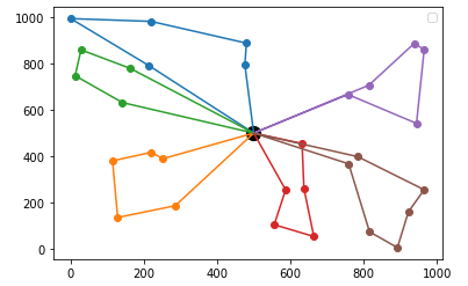
\includegraphics[width=\textwidth]{Gambar/Picture1.png}
\caption{MTSP dengan 6 klaster}
\end{subfigure}
\hfill
\begin{subfigure}[b]{0.48\textwidth}
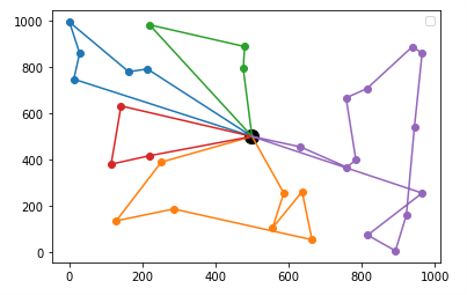
\includegraphics[width=\textwidth]{Gambar/Picture2.png}
\caption{MTSP dengan 5 klaster}
\end{subfigure}
\caption{Proses MTSP dengan klaster}
\label{fig:mtsp}
\end{figure}

\subsection{Algoritma}

Maulana menyebutkan dalam artikelnya algoritma adalah kumpulan perintah untuk menyelesaikan suatu masalah dan diselesaikan dengan cara sistematis, terstruktur dan logis \cite{maulana2017pembelajaran}. Algoritma digunakan untuk memecahkan permasalahan yang dialami oleh seorang pengguna program.

\subsection{Algoritma $k$-means}

$K$-means adalah jenis metode klasifikasi tanpa pengawasan yang mempartisi item data menjadi satu atau lebih klaster \cite{agusta2007k}. $K$-means mencoba untuk memodelkan suatu dataset ke dalam beberapa klaster sehingga item-item data dalam suatu klaster memiliki karakteristik yang sama dan memiliki karakteristik yang berbeda dengan klaster lainnya.

Menurut S Monalisa \cite{monalisa2018klasterisasi} tahapan mengklaster menggunakan algoritma \textit{k}-means adalah sebagai berikut.

\begin{enumerate}
	\item Menentukan banyak klaster
	\item Memilih beberapa \textit{centroid} secara acak sesuai banyak klaster
	\item Menghitung jarak titik ke \textit{centroid} dengan rumus \textit{Euclidean distance} seperti Persamaan (\ref{eq:euclidean}).
	\item Mengelompokkan titik-titik yang tersebar ke dalam klaster yang sama dengan titik \textit{centroid} paling dekat
	\item Memperbarui \textit{centroid} dengan menghitung nilai rata-rata nilai pada masing-masing klaster
	\item Melakukan iterasi sebanyak mungkin dengan kembali ke tahapan 3 sampai tidak ada perubahan klaster atau perubahan nilai \textit{centroid}
\end{enumerate}

\noindent Secara garis besar tahapan-tahapan algoritma genetika seperti diagram alir pada Gambar \ref{fig:flowkmeans}.

\begin{figure}[H]
\linespread{1}
\centering
%Definisi
\tikzstyle{bulat} = \tikzstyle{bulat} = [rectangle, rounded corners, minimum width=3cm, minimum height=1cm,text centered, draw=black, fill=red!30]
\tikzstyle{jajargenjang} = [trapezium, trapezium left angle=70, trapezium right angle=110, minimum height=1cm, text width=2cm, text centered, draw=black, fill=blue!30]
\tikzstyle{kotak} = [rectangle, minimum height=1cm, text width=3cm, text centered, draw=black, fill=orange!30]
\tikzstyle{belahketupat} = [diamond, text width=2cm, text centered, draw=black, fill=green!30]
\tikzstyle{garis} = [thick,->,>=stealth]

%Gambar
\begin{tikzpicture}
\node (1) [bulat] {Mulai};
\node (2) [jajargenjang, below of=1, yshift=-0.8cm]{Dataset, tentukan $n$ klaster};
\node (3) [kotak, below of=2, yshift=-1cm] {Pilih \textit{centroid} secara acak};
\node (4) [kotak, below of=3, yshift=-1cm] {Hitung jarak tiap titik ke \textit{centroid}};
\node (5) [kotak, below of=4, yshift=-2cm] {Pengelompokan berdasarkan jarak terkecil};
\node (6) [kotak, right of=5, xshift=+3.5cm] {Memindahkan \textit{centroid} ke tengah area};
\node (7) [belahketupat, above of=6, yshift=+2cm]{\textit{Centroid} berbeda?};
\node (8) [jajargenjang, right of=7, xshift=+3.5cm] {Hasil klaster};
\node (9) [bulat, below of=8, yshift=-1.5cm] {Selesai};

\draw [garis] (1) -- (2);
\draw [garis] (2) -- (3);
\draw [garis] (3) -- (4);
\draw [garis] (4) -- (5);
\draw [garis] (5) -- (6);
\draw [garis] (6) -- (7);
\draw [garis] (7) -- node[near start, color=black, yshift=+0.5cm]{Ya}(4);
\draw [garis] (7) -- node[near start, color=black, yshift=+0.5cm]{Tidak}(8);
\draw [garis] (8) -- (9);

\end{tikzpicture}
\caption{Diagram alir tahapan $k$-means}
\label{fig:flowkmeans}
\end{figure}

\subsection{\textit{Centroid}}

\textit{Centroid} adalah nilai yang dijadikan sebagai titik awal dimulainya sebuah pengelompokan (\textit{clustering}) pada algoritma $k$-means \cite{retno2019peningkatan}. Untuk melakukan pengelompokan data, dimulai dengan menghitung jarak dari setiap titik tujuan menuju ke setiap titik \textit{centroid} sebagai awal pembentukan klaster, setelah itu titik-titik tujuan akan dikelompokkan menurut titik klaster terdekatnya. Dalam langkah tersebut akan dihitung titik-titik \textit{centroid} yang baru menggunakan nilai rata-rata titik dari tiap klaster.

\subsection{Algoritma Genetika}

Pada artikel Hermanto disebutkan bahwa algoritma genetika adalah algoritma yang digunakan untuk mencari solusi suatu permasalahan dengan cara yang lebih alami yang terispirasi dari teori evolusi  \cite{hermawanto2003algoritma}. Dalam hal ini, algoritma genetika dapat juga digunakan untuk pencarian sebuah rute terpendek dalam sebuah kasus perjalanan.

Menurut Armanda RS \cite{armanda2016penerapan} dalam artikelnya menyampaikan penyelesaian masalah menggunakan algoritma genetika memerlukan beberapa tahapan sebagai berikut:

\begin{enumerate}
	\item Bangkitkan populasi, dalam penelitian ini yang digunakan adalah data yang telah diklaster menggunakan algoritma \textit{k}-means
	\item Melakukan reproduksi dengan \textit{crossover} dan mutasi pada pembentukan awal populasi
	\item Menyeleksi menggunakan metode \textit{elitism}
	\item Menentukan nilai \textit{fitness} agar mendapatkan solusi akhir yang optimal
	\item Iterasi dilakukan untuk generasi berikutnya.
\end{enumerate}

\noindent Secara garis besar tahapan-tahapan algoritma genetika seperti diagram alir pada Gambar \ref{fig:flowag}.

\begin{figure}[H]
\centering
\linespread{1}
%Definisi
\tikzstyle{bulat} = \tikzstyle{bulat} = [rectangle, rounded corners, minimum width=3cm, minimum height=1cm,text centered, draw=black, fill=red!30]
\tikzstyle{jajargenjang} = [trapezium, trapezium left angle=70, trapezium right angle=110, text width=2cm, minimum height=1cm, text centered, draw=black, fill=blue!30]
\tikzstyle{kotak} = [rectangle, minimum height=1cm, text width=3cm, text centered, draw=black, fill=orange!30]
\tikzstyle{kotak2} = [rectangle, minimum height=1cm, text width=5cm, text centered, draw=black, fill=orange!30]
\tikzstyle{belahketupat} = [diamond, minimum width=3cm, minimum height=1cm, text centered, draw=black, fill=green!30]
\tikzstyle{garis} = [thick,->,>=stealth]
%Gambar
\begin{tikzpicture}
\node (S) [bulat] {Mulai};
\node (in) [jajargenjang, below of=S, yshift=-0.8cm]{Dataset};
\node (pop) [kotak2, below of=in, yshift=-0.8cm] {Bangkitkan Populasi Awal};
\node (fit) [kotak, below of=pop, yshift=-0.8cm] {Hitung \textit{fitness}};
\node (sel) [kotak, right of=fit, xshift=+3.5cm] {Seleksi};
\node (cross) [kotak, below of=sel, yshift=-0.8cm] {\textit{Crossover}};
\node (mut) [kotak, below of=cross, yshift=-0.8cm] {Mutasi};
\node (opt) [belahketupat, left of=mut, xshift=-3.5cm] {\textit{fitnes} sama?};
\node (out) [jajargenjang, below of=opt, yshift=-1.7cm]{Kromosom Optimal};
\node (E) [bulat, below of=out, yshift=-0.8cm] {Selesai};
\draw [garis] (S) -- (in);
\draw [garis] (in) -- (pop);
\draw [garis] (pop) -- (fit);
\draw [garis] (fit) -- (sel);
\draw [garis] (sel) -- (cross);
\draw [garis] (cross) -- (mut);
\draw [garis] (mut) -- (opt);
\draw [garis] (opt) -- node[near start, color=black, xshift=+0.5cm]{Ya}(out);
\draw [garis] (opt) -- node[near start, color=black, xshift=+0.5cm]{Tidak}(fit);
\draw [garis] (out) -- (E);
\end{tikzpicture}
\caption{Diagram alir tahapan algoritma genetika}
\label{fig:flowag}
\end{figure}

\subsection{\textit{Fitness}}
\textit{Fitness} adalah suatu ukuran yang dijadikan acuan untuk mengetahui baik atau tidaknya suatu individu atau bisa disebut nilai dari fungsi tujuan \cite{basuki2003strategi}. Tujuan dari penggunaan algoritma genetika adalah untuk mengoptimalkan nilai tujuan dengan cara mencari nilai fitness yang paling maksimal atau minimal. Nilai \textit{fitness} suatu kromosom menggambarkan kualitas kromosom dalam populasi tersebut. Seperti dalam penelitian ini adalah mencari jarak yang paling minimal maka nilai \textit{fitness}nya yang dicari adalah yang paling minimal juga. Untuk mengghitung nilai \textit{fitness} dapat menggunakan Persamaan \ref{eq:fitness}.

	\begin{equation}
    fit=\sum (d_{ij})
    \label{eq:fitness}
    \end{equation}
    
    Keterangan:
    \begin{itemize}
	\item $d_{ij}$ adalah jarak \textit{Euclidean Distance} dapat dilihat pada Persamaan \ref{eq:euclidean}
    \end{itemize}
	
\subsection{\textit{Euclidean distance}}

\textit{Euclidean distance} pertama kali diperkenalkan oleh ilmuan Yunani. Jarak \textit{Euclidean} merupakan metode yang digunakan untuk menghitung jarak antara dua buah titik pada dua dimensi atau tiga dimensi \cite{widodo2018penerapan}. Untuk menghitung jarak \textit{Euclidean} dapat dilihat pada Persamaan \ref{eq:euclidean}.
       
    \begin{equation}
	d_{ij}=\sqrt{\left( x_j-x_i \right)^{2}+\left( y_j-y_i \right)^{2}}
	\label{eq:euclidean}
	\end{equation}
	
	Keterangan:
	\begin{itemize}
	\item $d_{ij}$ adalah nilai jarak pada titik $i$ ke titik $j$
	\item $x_i$ dan $y_i$ adalah nilai koordinat $x$ dan $y$ pada titik $i$
	\item $x_j$ dan $y_j$ adalah nilai koordinat $x$ dan $y$ pada titik $j$
	\end{itemize}

\subsection{\textit{Crossover}}
\textit{Crossover} atau persilangan adalah operator dari algoritma genetika yang melibatkan dua induk untuk membentuk kromosom baru menurut Hardi, dkk. pada artikelnya \cite{hardi2014analisis}. Dalam langkah ini dilakukan dengan cara menukar sebagian gen pada kromosom induk pertama dengan gen pada kromosom induk kedua seperti pada Gambar \ref{fig:crossover}. Proses \textit{crossover} tersebut diterapkan pada setiap individu dengan probabilitas \textit{crossover} ($p_c$) yang telah ditentukan. Jika diterapkan \textit{crossover} keturunan didapatkan dari kromosom-kromosom induk. Jika \textit{crossover} tidak diterapkan, satu induk dipilih secara acak dengan $p_c$ yang sama dan diduplikasi menjadi anak.

\begin{figure}[H]
  \centering
  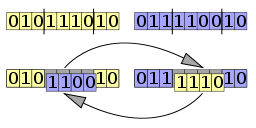
\includegraphics[width=0.5\textwidth]{Gambar/crossover.png}
  \caption{Proses \textit{crossover}}
  \label{fig:crossover}
\end{figure}

\subsection{Mutasi}
Mutasi atau \textit{mutation} adalah operator yang digunakan untuk mengubah gen-gen yang terdapat dalam kromosom. Model dalam proses ini sebagaimana yang terjadi dalam kehidupan alam \cite{rovie2014genetic} seperti pada Gambar \ref{fig:mutasi}. Dalam proses mutasi akan dibangkitkan sebuah bilangan acak sebagai Probabilitas mutasi ($p_m$) yang sangat kecil. Mutasi diterapkan dengan tujuan untuk memperoleh nilai \textit{fitness} yang lebih baik dari sebelumnya, dan lama-kelamaan akan menjadi solusi optimum yang diinginkan.

\begin{figure}[H]
  \centering
  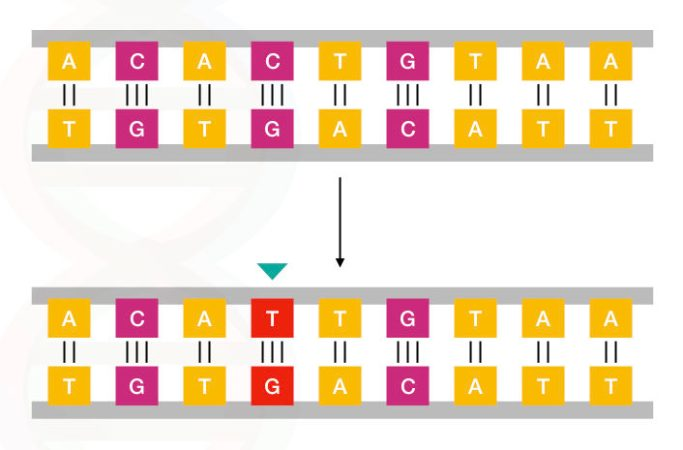
\includegraphics[width=0.5\textwidth]{Gambar/mutasi.jpg}
  \caption{Proses mutasi}
  \label{fig:mutasi}
\end{figure}